\documentclass{ltjsreport}

\usepackage{luatexja-fontspec}
\usepackage[ipa]{luatexja-preset}

% 参考文献リストの設定
% 参考文献はreferences.bibに記述する
\usepackage[backend=biber]{biblatex}
\addbibresource{references.bib}

\title{温度感受性イオンチャネルタンパク質の物性と分子機能}
\author{名古屋大学理学研究科理学専攻\\杉浦航}
\date{\today}

\begin{document}

% 表紙
\maketitle

\chapter*{概要}
生物は温度変化に敏感に反応し、これに対応することで生存に必要な生理機能を維持している。
TRP チャネルは、温度変化を感知する膜タンパク質であり、その変化によりイオンチャネルが開口し、カチオンが細胞内に流入して電位が変化し、電気信号が生成される。
最新のクライオ電子顕微鏡と分子動力学シミュレーション技術を用いて、TRP チャネルの立体構造とその機能について詳細な解析が行われており、
例えば TRPV3 は温度変化を感知するタンパク質全体に散在するドメインを介して二段階の構造変化を示すことが明らかにされている。
しかし、これらのドメインがお互いにどのように相互作用してイオンチャネルの協同的な開口を調節しているのか、未だに解明されていない。

そこで本研究では、TRPV3 チャネルの閉じた構造と開いた構造における熱流解析を実施し、アミノ酸残基間の相互作用を特徴づけることでそれらを比較する。

まず、分子動力学シミュレーションを行い分子のトラジェクトリを取得し、熱流解析、熱伝導度の計算を行った。
熱流解析には、当研究室で開発した curpを使用したが、大規模なタンパク質に対しては計算時間が非常に大きくなる課題があった。
したがって、計算時間を短縮するための新しい手法を開発した。具体的には、座標データのアクセス時間を最適化し、時間的局所性を高めるようにプログラムを改良した。
その結果、計算時間を最大40\%短縮できることが確認された。閉じた構造と開いた構造における熱流解析の比較結果については論文と当日の発表で紹介する。


% 目次
\tableofcontents
\clearpage

\chapter{序論}
\section{はじめに}

タンパク質はアミノ酸が多数繋がって構成されている高分子化合物であり、タンパク質全体が分子機械として働く。しかしこのアミノ酸単位やアミノ酸間の相互作用という”部分”としての局所的挙動とドメイン単位やタンパク質という”全体”としての大域的挙動には時空間の大きな隔たりがある。
それが顕著に表れている具体的な話でいうと、タンパク質のアロステリー現象が挙げられる。
タンパク質のアロステリー現象は、リガンド結合や外部刺激によって生じる構造変化が刺激受容部位から遠隔の活性部位に影響を及ぼす現象であり、そのメカニズム解明は生命現象の理解と創薬研究の中心的的題の一つである。
%参考文献:アロステリーの特性
%2009「アロステリーと協同性の再考」
%https://onlinelibrary.wiley.com/doi/10.1110/ps.03259908
アロステリーはタンパク質の機能を制御する重要な特性であり\cite{Cui2009}、リガンド結合など外部刺激のシグナルが残基間相互作用を介して活性部位に伝達する仕組みを提供する。
この過程の特徴を2点挙げる。\\
1.活性部位がサブÅ~数十Å離れた場所でのリガンド結合や微小環境の摂動を総じた情報を受け取る点。\\
2.ピコ秒オーダーの残基間エネルギー移動過程\cite{Lim1996}がミリ秒以上のアロステリック遷移\cite{Changeux2005}を引き起こす点。
つまりこの過程は、サブピコ秒からミリ秒の時間スケールにわたるダイナミクスと、サブÅから数十Åの空間スケールの相互作用が連動して行われることが興味深い点であり大きな謎\cite{Fenton2008}となっている。
%参考文献:アロステリー、時間スケールと空間スケール
%2005「シグナル伝達のアロステリック機構」
%https://www.science.org/doi/abs/10.1126/science.1108595
%大きな謎
%2008「アロステリー:「生命の第二の秘密」の図解による定義」
%https://www.sciencedirect.com/science/article/pii/S0968000408001643
この離れた場所間のコミュニケーションを解明する一つの方法として、グラフ理論を用いたアプローチが注目されている。
グラフ理論は、分子内の残基間の相互作用をネットワークとして表現し、複雑な動的挙動を解析するための強力なツールとして広く利用されてきた\cite{Doncheva2011}\cite{Martin2011}\cite{Doncheva2012}。
%参考文献:グラフ理論
%2011「タンパク質構造の残基ネットワークの解析と可視化」
%https://www.cell.com/trends/biochemical-sciences/abstract/S0968-0004(11)00013-2?_returnURL=https%3A%2F%2Flinkinghub.elsevier.com%2Fretrieve%2Fpii%2FS0968000411000132%3Fshowall%3Dtrue
%2011「RING: タンパク質構造における相互作用残基、進化情報、エネルギーのネットワーク化」
%https://academic.oup.com/bioinformatics/article/27/14/2003/193801?login=false
%2012「生物学的ネットワークとタンパク質構造のトポロジー解析とインタラクティブな可視化」
%https://www.nature.com/articles/nprot.2012.004
タンパク質を構造ネットワークとしてモデル化すると、シグナル伝達機構を解釈しやすくなる。
そのようなモデルは、ネットワーク内の最短経路の存在の重要性を強調\cite{Ghosh2007}しており、それらが離れた部位間での効率的な情報伝達に寄与していることを示している。
%参考文献:最短経路
%2007「分子動力学シミュレーションと構造ネットワーク解析によるメチオニルtRNA合成酵素のコミュニケーション経路の研究
%https://www.pnas.org/doi/full/10.1073/pnas.0704459104
また、その前提のもとで、高い中心性を持つ残基\cite{amitai2004}やネットワーク上における最短経路上によく現れる残基\cite{delsol2006}を解析することで、機能的残基を同定してきた。
%参考文献:中心性
%2004「タンパク質構造のネットワーク解析により機能残基を特定」
%https://www.sciencedirect.com/science/article/pii/S0022283604013592
%参考文献:最短経路
%2006「ネットワーク通信における短い経路を維持するために重要な残基がタンパク質のシグナル伝達を媒介する」
%https://www.embopress.org/doi/full/10.1038/msb4100063
実際にこれらの残基はタンパク質の折りたたみにおける重要なアミノ酸や酵素ファミリーの活性部位残基であると関連付けられている。

しかし、残基間エネルギー移動過程とアロステリック遷移の時間スケールの違いを考慮すると、単純な「最短経路モデル」だけではアロステリーの情報伝達を十分に説明できない可能性がある。
実際に、残基集団の協調的な運動\cite{Kornev2015}や、複数経路の存在\cite{delSol2009}を示す文献もあり、この視点はアロステリーのより現実的で包括的な理解を提供する可能性がある。
%複数経路の論文
%2009「アロステリック機能調節の起源:複数の既存経路」
%https://www.sciencedirect.com/science/article/pii/S0969212609002500?via%3Dihub
%参考文献:バイオリンモデル
%2015「タンパク質キナーゼにおけるダイナミクス駆動型アロステリー」
%https://www.cell.com/trends/biochemical-sciences/fulltext/S0968-0004(15)00166-8

本研究では、アロステリーの解析対象として$\beta_2$アドレナリン受容体($\beta_2$AR)を選定した。
まず分子動力学(MD)シミュレーションを用いて得られたinactive状態とactive状態におけるトラジェクトリー解析から、残基間距離を反映したネットワークを構築した。
さらに、Louvain法\cite{Blondel2008}によるコミュニティ検出を適用し、コミュニティによるシグナル伝達機構を定量的に解析した。

その結果、active状態において新たなコミュニティの生成が有意に認められ、これがシグナル伝達において重要な役割を果たすことが示唆された。
また、膜タンパク質内のエネルギー的に保存された水分子\cite{Angel2009}が果たす役割を確認した。

\section{$\beta_2$アドレナリン受容体($\beta_2$AR)}
\label{sec:b2ar}

\subsubsection{基本情報}
$\beta_2$アドレナリン受容体($\beta_2$AR)は、Gタンパク質共役受容体(GPCR)の一種である。
GPCRは細胞膜に存在する膜タンパク質であり、ホルモンや神経伝達物質などの細胞外刺激を認識し、それを細胞内のシグナルに変換する役割を担っている。
また、視覚、嗅覚、味覚といった感覚にも関与し、生体内の多様なシグナル伝達経路において中心的な役割を果たしている。
GPCRは7回膜貫通構造を持つことが特徴であり、各膜貫通ヘリックス(TM1からTM7)は、細胞外ループ(ECL)と細胞内ループ(ICL)を介して他のヘリックスと連結されている。
この構造により、細胞外でのリガンド認識と細胞内でのシグナル伝達を効率的に行うことが可能となる。

%画像、リガンドとgproteinの色を変えるべき?、TM1-TM7/ECL-ICLを示す
\begin{figure}[htbp]
    \centering
    \begin{subfigure}{0.45\textwidth} % 各図の幅を調整
      \centering
      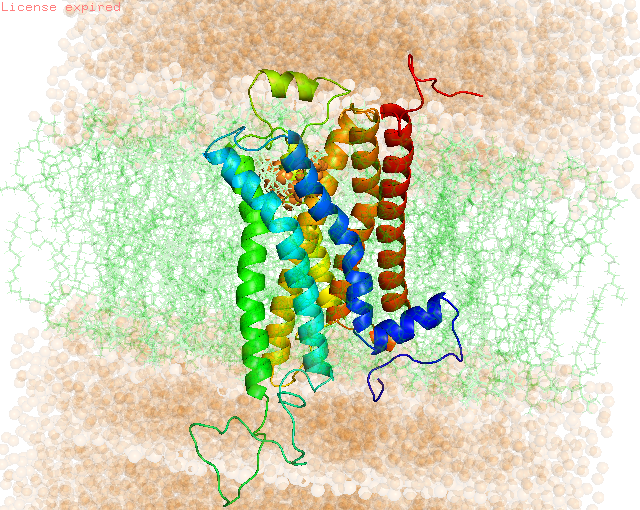
\includegraphics[width=\textwidth]{inactive_system-all.png}
      \caption{$\beta_2$ARのinactive状態。}
      \label{fig:inactive_system}
    \end{subfigure}
    \hspace{0.05\textwidth} % 図の間のスペース
    \begin{subfigure}{0.45\textwidth}
      \centering
      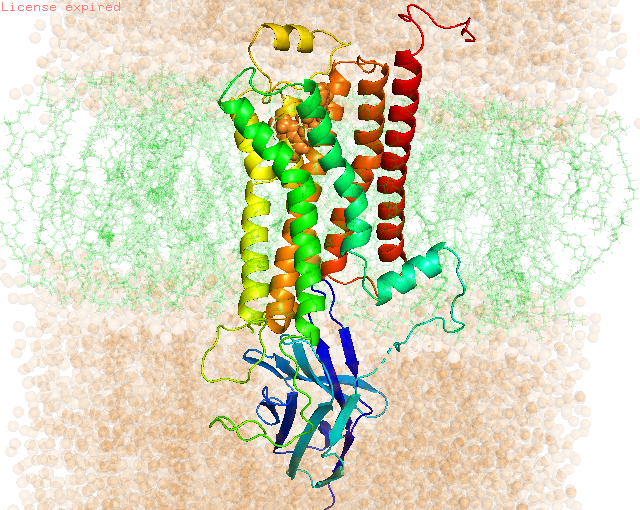
\includegraphics[width=\textwidth]{active_system-all.png}
      \caption{$\beta_2$ARのactive状態。}
      \label{fig:active_system}
    \end{subfigure}
    \caption{$\beta_2$ARのinactive状態とactive状態の初期構造。}
    \label{fig:system-all}
  \end{figure}

膜タンパク質の構造データは、Protein Data Bank(PDB)から取得した。
$\beta_2$ARの不活性状態として2RH1\cite{cherezov2007},活性状態として3P0G\cite{rasmussen2011}を用いた。
%2RH1の構造情報2007
%https://www.science.org/doi/10.1126/science.1150577
%3P0Gの構造情報2011
%https://www.nature.com/articles/nature09648

\subsubsection{活性化に伴う構造的変化}
$\beta_2$ARのinactive状態からactive状態への活性化は、リガンド結合部位に結合したアゴニストによって引き起こされる。
すると受容体が活性化され、特にGsといったGタンパク質の結合が促進される。
Gsはヘテロ三量体型タンパク質であり、その活性化により細胞内でアデニル酸シクラーゼが刺激され、cAMP(サイクリックAMP)の産生が増加する。
この過程\cite{philip2007}を通じて、細胞内のシグナル伝達経路が活性化される。
%参考文献:GPCRのシグナル伝達機構
%2007「G タンパク質共役受容体とそれに対応する G タンパク質を介したシグナル伝達は、化学量論的に制限されたモデルに従う」
%https://www.sciencedirect.com/science/article/pii/S002192582087389X

%詳細の構造と、リガンド・gタンパク質結合部位を示す
β2ARのリガンド結合部位は膜貫通ヘリックス(TM)の間に位置し、細胞外の刺激を感知する。
一方で、Gタンパク質との結合は細胞内ループおよび細胞質側ドメインを介して行われる。


アゴニストが結合した$\beta_2$ARは、顕著な構造変化を引き起こす\cite{rasmussen2011crystal}ことがわかっている。
%参考文献:β2ARの構造変化
%2011「β2アドレナリン受容体-Gsタンパク質複合体の結晶構造」
%https://www.nature.com/articles/nature10361
主な変化として以下が挙げられる:
\begin{enumerate}
    \item \textbf{TM6の移動}: TM6の細胞質側末端が、約14Å外側に移動する。この移動により、Gタンパク質が結合するための空間が確保される。
    \item \textbf{TM5の変化}: TM5の細胞質側末端部分において、αヘリックスの延長が観察される。これにより、シグナル伝達に関与する構造が再編成される。
\end{enumerate}

\subsubsection{活性化に関わる重要な残基}
$\beta_2$ARの活性化において、特定のモチーフ\cite{nygaard2009ligand}\cite{lee2013mapping}が重要な役割を果たしていることが知られている。

%参考文献:モチーフ
%2009「7TM受容体構造におけるリガンド結合とマイクロスイッチ」
%https://www.sciencedirect.com/science/article/pii/S0165614709000546
%参考文献:モチーフ
%2013「Gタンパク質共役受容体の分子内シグナル伝達のマッピング」
%https://onlinelibrary.wiley.com/doi/10.1002/prot.24451
%参考文献:保存水
%2009「保存された水はファミリーA(ロドプシン様)Gタンパク質共役受容体の構造的および機能的活性化を媒介する」
%https://www.pnas.org/doi/10.1073/pnas.0903545106
モチーフとは、タンパク質中の特定の機能に関連する保存されたアミノ酸配列のことであり、GPCRではアロステリックシグナル伝達やコンフォメーション変化を介して受容体の機能を調節する。
$\beta_2$ARを含むクラスA GPCRでは、以下の4つの主要な保存モチーフ(DRY、CWxP、NPxxY、PIF)と「イオンロック」が重要な役割を果たしている。

\begin{itemize}
  \item \textbf{DRYモチーフ}  
  TM3の細胞質側領域に位置し、Asp(D)-Arg(R)-Tyr(Y)から構成される。inactive状態ではTM6のGluとイオンロックを形成し、構造を安定化させている。一方、active状態ではイオンロックが解除され、Gタンパク質との結合が可能になる。

  \item \textbf{CWxPモチーフ}  
  TM6のリガンド結合ポケットの底部に位置し、Cys(C)-Trp(W)-任意の残基(x)-Pro(P)から構成される。inactive状態ではTrpがリガンド結合ポケットを開いた状態を維持しているが、active状態ではTrpが「トグルスイッチ」として機能し、ポケットを閉じる役割を果たす。

  \item \textbf{NPxxYモチーフ}  
  TM7の細胞質側に位置し、Asn(N)-Pro(P)-任意の残基(xx)-Tyr(Y)から構成される。このモチーフにおけるTyrは、不活性状態と活性状態で異なる立体配座間を回転することで、構造の変化を媒介する。

  \item \textbf{PIFモチーフ}  
  TM4、TM5、TM6にまたがる位置に存在し、Pro(P)-Ile(I)-Phe(F)から構成される。このモチーフにおけるPheはスイッチとして機能し、活性化時に異なる立体配座間で方向を変えることで重要な役割を果たす。

  \item \textbf{イオンロック}  
  TM3とTM6の間に位置している。不活性状態ではイオンロックが形成され、構造を安定化させているが、活性化時にはこのロックが解除され、GPCRの完全な活性化を促進する。
\end{itemize}


また水分子も、生物学的システムにおいて重要な役割を果たすことが知られており、特にGPCRの活性化メカニズムにも深く関与している。
ロドプシンをはじめとするGPCRにおいて、保存された水は活性化過程においてアロステリックを仲介する機能を果たすことが示されている\cite{angel2009conserved}。
$\beta_2$ARにおいても、膜貫通ドメイン内にはいくつかの保存された水分子が確認され、これらの水分子はアロステリックシグナル伝達に関与していると考えられる。
らに、inactive状態とactive状態それぞれのβ2AR構造間で水分子の位置や配置がどのように変化するかを比較することで、水の動態が受容体の機能に与える影響を明らかにすることができる可能性がある。

そこで本研究でも、モチーフと保存された結晶水がコミュニティ構造に与える影響を解析し、シグナル伝達機構における役割を明らかにすることを目指す。


\chapter{材料と方法}
% 方法と材料を述べる
% 今回の研究では、次のテクニックを使った。
% - RMSD
% - RMSF
% - Thermal conductivity by curp
%   - 熱流の理論式
%   - 熱伝導度の理論式
% - MD simulation
%   - AMBER
%   - PME
%   - NPgT
%   - NPT
%   - minimization
%   - equilibration
%   - production
%   - NVE

% アウトライン
% - 熱伝導度の理論を説明する
%   - 熱伝導度の計算方法を説明する
% - 熱伝導度を計算するための準備としての、分子動力学シミュレーションの方法を説明する
%   - エネルギー最小化
%   - 熱平衡化
%   - sampling
%   - NVE

\section{熱伝導度の解析}
% - 熱伝導度と熱流について述べる
本研究では、先行研究が示したEEN、\Delta EEN、r\Delta EENの概念\autocite{ishikura2015,ota_energy_2019,poudel_energy_2022}を
熱流解析に応用して、TRPV3の活性化と調節における構造的および機能的ダイナミクスを明らかにする。
なお、本研究の目的を達成するには熱流にこだわらずEnergy fluxやエネルギー伝導度を用いた方法を用いてもよいが
熱流から計算される熱伝導度は、実験的に測定することができるというメリットがあるため、本研究では熱流を用いた手法を用いることにした。

先行研究でエネルギー流ではなくエネルギー伝導度を用いていたことにならい、本研究でも熱流ではなく熱伝導度を用いて解析した。
ここで、熱伝導度と熱流について簡単に説明する。

% TODO: 改善。
熱伝導度$\lambda$は平衡状態において。

\begin{equation}
  \label{eq:thermal_conductivity}
  \lambda = \frac{1}{3Vk_B T^2} \int_{0}^{\infty} \left\langle
    \bm{h}(0) \cdot \bm{h}(t)
  \right\rangle dt
\end{equation}

ここで$\mathbf{h}$は熱流を表す。\autocite{mcquarrie_statistical_2000}

熱流$\mathbf{h}$をこう定義する。

\begin{equation}
  \label{eq:heat_flow}
  \bm{h} \equiv \frac{d}{dt} \left\{
    \sum_{i=1}^{N} \bm{r}_i \cdot E_i
  \right\} = \sum_{i=1}^{N} \left\{
    \frac{d\bm{r_i}}{dt}E_i + \bm{r_i}\frac{dE_i}{dt}
  \right\}
\end{equation}

ここで、右辺の $\frac{dE_i}{dt}$は

\begin{equation}
  \label{time_derivative_of_energy}
  \frac{dE_i}{dt} = \sum_{j=1}^{N} \frac{1}{2} \bf{F}_{ij} \cdot (\bf{v}_i + \bf{v}_j)
\end{equation}

と展開できる\autocite{leitner_mapping_2018}。
また、タンパク質中の原子の運動は著しく制限されるため$\frac{d\bm{r_i}}{dt}E_{i}$が十分小さいと考えて無視すれば、
式\ref{eq:heat_flow}は次のように変形できる。\autocite{yamatoComputationalStudyThermal2022,oai:nagoya.repo.nii.ac.jp:02007698}

\begin{align}
  % \label{eq:heat_flow_expanded}
  \bm{h} &= \sum_{i=1}^{N} \left\{
              \bm{r_i}\sum_{j=1, j \neq i }^{N} \frac{1}{2} \bf{F}_{ij} \cdot (\bf{v}_i + \bf{v}_j)
            \right\} \\
         &= \sum_{i=1}^{N} \sum_{j>i}^{N}
              (\bm{r_i} - \bm{r_j}) \frac{1}{2} \bf{F}_{ij} \cdot (\bf{v}_i + \bf{v}_j) \\
         &= \sum_{(i, j)}
              (\bm{r_i} - \bm{r_j}) \frac{1}{2} \bf{F}_{ij} \cdot (\bf{v}_i + \bf{v}_j) \\
         &= \sum_{(i, j)}
              \bm{h}_{ij}
\end{align}

ここで、一行目から二行目への式変形には $\bf{F}_{ij} = - \bf{F}_{ij}$を用いた。
ここで得られた熱流$\bm{h}_{ij}$を使い、残基A、B間の熱流$\bm{h}{AB}$を次のように定義する。

\begin{equation}
  \label{eq:heat_flow_between_residues}
  \bm{h}_{AB} = \sum_{\substack{(i, j) \\ i \in \rm{A}, j \in \rm{B}}} \bm{h}_{ij}
\end{equation}

\section{分子動力学シミュレーション}

熱伝導度を計算するためには、NVEアンサンブルでの分子動力学シミュレーションを行う必要がある。
そのため本研究では、モデリング、構造最適化、熱平衡化、サンプリング、解析の5つのステップを踏んで熱伝導度の計算を行った。

\subsection{モデリング}
開構造として7MIO、% FLOW_ID = 13, structure_id = 11
閉構造として7MIN  % FLOW_ID = 11, structure_id = 9 
を用いた。\autocite{noauthor_7mio_nodate, noauthor_7min_nodate, nadezhdinStructuralMechanismHeatinduced2021}
それぞれの構造について、CHARMM-GUIのInput generator\autocite{jo_charmmgui_2008, lee_charmm-gui_2016}を用いて、リン脂質二重膜にタンパク質を挿入して、シミュレーションボックスを作成した。
なお、今後開構造の7MIOを「\openFortyTwo」、閉構造の7MINを「\closeFortyTwo」と呼ぶことにする。

CHARMM-GUIを用いて、次のように系を作成した。
まず、\openFortyTwo は残基番号77から112までの残基はモデリングされていなかったため、残基番号113以降の構造情報のみを用いた。
次に、PDBデータに含まれていたタンパク質以外の分子についてはあらかじめすべて除去した。
また、両方のモデルについて、タンパク質分子に対して pH 7.0 でプロトン化した。
続けて、作成したモデルをリン脂質二重層に挿入した。
% メモ: 脂質の名前に自信がない。
% メモ: newcommandで定義しているので、後で変更するときは定義場所だけ変更すればよい。
% POPC
%  - 1-palmitoyl-2-oleoyl-sn-glycero-3-phosphocholine, https://en.wikipedia.org/wiki/POPC
% POPE
%  - 1-palmitoyl-2-oleoyl-sn-glycero-3-phosphoethanolamine, https://avantilipids.com/product/850757
%  - palmitoyloleoyl-phosphatidylethanolamine, https://www.ncbi.nlm.nih.gov/pmc/articles/PMC1305115/
%  - 1-Palmitoyl-2-oleoylphosphatidylethanolamine, https://pubchem.ncbi.nlm.nih.gov/compound/1-Palmitoyl-2-oleoylphosphatidylethanolamine
%  - 1-palmitoyl-2-oleoyl-phosphatidylethanolamine, https://pubs.acs.org/doi/10.1021/bi060937y
脂質二重層の構成分子は、\molNamePOPC (POPC)、\molNamePOPE (POPE)、\molNameCHOL (CHOL)を使い、これらの分子をPOPC:POPE:CHOL=2:1:1の比率で混合した。
最後に、水分子とNaClイオンを加えて系の電荷を中和した。NaClイオンは0.15 Mの濃度になるように追加した。
シミュレーションパッケージAMBER 22\autocite{case_amber_2023}を使ったため、ポテンシャル関数としてAMBER\autocite{pearlman_amber_1995}を利用した。
ポテンシャル関数の各パラメータは、
タンパク質の原子にはff19SB\autocite{tian_ff19sb_2020}、
脂質の原子にはLipid21\autocite{dickson_lipid21_2022}、
水分子にはOPC水モデル\autocite{izadi_building_2014}を用いた。
系には3次元の周期境界条件を設定した。
系を作成した後の系の大きさを表\ref{tab:system_size}に示す。

\begin{table}[!ht]
  \centering
  \caption{シミュレーションに用いた系の大きさ}
  \begin{tabular}{lll}
    \hline
    モデル名        & 原子数  & ボックスの大きさ(x, y, z) \\
    \hline 
    \openFortyTwo  & 1183281 & 250.19627, 250.19627, 161.529 \\ 
    \closeFortyTwo & 1206767 & 250.14921, 250.14921, 164.691 \\ 
  \end{tabular}
  \label{tab:system_size}
\end{table}

\subsection{シミュレーション}
作成したモデルは、以下の手続きによりシミュレーションを行った。シミュレーションには、Particle Mesh Ewald法を用いた。
% 粒子として取り扱う距離を cut = 9 [A]とした。

はじめに、構造最適化を行った。構造最適化は3つのステップに分けて行った。
最初のステップでは、水以外の原子に対してrestraintをかけて、水の構造、並びを最適化した。
次のステップでは、タンパク質の原子に対してrestraintをかけて、水と脂質の構造を最適化した。
最後のステップでは、すべてのrestraintを外して、全体の構造を最適化した。
各ステップにおいて、最初の2500ステップで再急降下法によるエネルギー最小化を行い、次の2500ステップで共役勾配法によるエネルギー最小化を行った。

次に、熱平衡化を行った。
熱平衡化は大きく分けて2つのステップに分けて行った。
% 1. T = 10K で開始。NVT. 初期速度はマクスウェル分布で与える。1.mdinと2.mdinを使って、dt = 1 fsで125000 + 125000 = 250 psのシミュレーションの中で10 K -> 300Kまで上げる。
% 2. NPgT. 125000 steps, dt = 1 fs. 3.mdin
% 3. NPgT. 250000 steps, dt = 2 fs. 4.mdin
% 4. 
初めに、NVTアンサンブルで系の温度を上げた。初期速度は温度$T = 10 \rm{[K]}$のマクスウェル分布に従って与え、250 $\rm{ps}$で温度を$T = 315.15 \rm{[K]}$まで上昇させた。
次に、NP\gamma Tアンサンブルで平衡化を行った。
NP\gamma Tアンサンブルでは、温度、膜の表面張力、系の総数が一定になるようにシミュレーションを行う。% TODO: NPgTの説明を書く
詳細なシミュレーション条件は、表\ref{tab:simulation_condition}に示す。

% TODO: restraintについて記述する。
\begin{table}[!ht]
  \centering
  \caption{シミュレーション条件}
  \begin{tabular}{lllll}
    \hline
    ステップ & \Delta t [fs] & 時間 [ps] & アンサンブル & 温度 [T] \\
    \hline
    1       & 1              & 125       & NVT         & 10 $\rightarrow$ 100 \\
    2       & 1              & 125       & NVT         & 100 $\rightarrow$ 315.15 \\
    3       & 1              & 125       & NP\gamma T  & 315.15 \\
    4       & 2              & 500       & NP\gamma T  & 315.15 \\
    5       & 2              & 500       & NP\gamma T  & 315.15 \\
    6       & 2              & 500       & NP\gamma T  & 315.15 \\
  \end{tabular}
  \label{tab:simulation_condition}
\end{table}

続いて、NP\gamma Tシミュレーションによるサンプリングを行った。
熱平衡化の最後のステップと同じ、ただしrestraintを外した状態で10 nsのシミュレーションを実行した。
最後の5 nsの中で、各500 psごとに座標と速度を保存し、次のNVEのシミュレーションの初期状態として用いた。

最後にNVEシミュレーションによるサンプリングを行った。
初期状態として、NP\gamma Tシミュレーションによるサンプリングで得られた座標と速度を用いた。
保存した座標と速度のうち、5つを使って\Delta t = 1 fs、1 nsのシミュレーションを実行した。
シミュレーション中、各10 fsごとにトラジェクトリを保存した。

\section{熱伝導度の解析}

NVEシミュレーションによって得られたトラジェクトリを用いて、熱伝導度を計算した。
熱伝導度の計算には、CURP\autocite{ishikura_energy_2015,ota_energy_2019,yamatoComputationalStudyThermal2022,wangSiteselectiveHeatCurrent2023} を用いた。


なお、今回の研究を遂行するにあたり、熱流の計算速度を改善する必要があったため、改良を施したので次節で述べる。

\subsection{CURPの改良}\label{sec:curp}



\chapter{結果}
\section{分子動力学(MD)シミュレーション}

%MDの信頼性、同定されたDOWSERによる結晶水/保存されている結晶水の画像と説明
$\beta_2$ARのinactive状態active状態双方で1000psトラジェクトリを計10本取得した。
また保存された結晶水はinactive状態で7個、active状態で5個同定され、
その位置は図\ref{fig:water-all}に示す。

\begin{figure}[htbp]
    \centering
    \begin{subfigure}{0.45\textwidth} % 各図の幅を調整
      \centering
      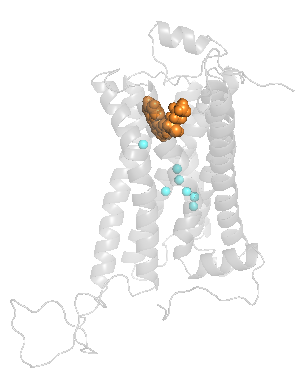
\includegraphics[width=\textwidth]{inactive_saved_water.png}
      \caption{$\beta_2$ARのinactive状態における保存された結晶水。}
      \label{fig:inactive_water}
    \end{subfigure}
    \hspace{0.05\textwidth} % 図の間のスペース
    \begin{subfigure}{0.45\textwidth}
      \centering
      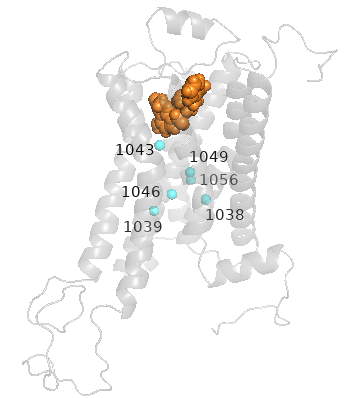
\includegraphics[width=\textwidth]{active_saved_water.png}
      \caption{$\beta_2$ARのactive状態における保存された結晶水。}
      \label{fig:active_water}
    \end{subfigure}
    \caption{保存された結晶水}
    \label{fig:water-all}
  \end{figure}

%先行研究との比較

\section{$\beta_2$ARのinactiveおよびactive状態のコミュニティ検出}

\subsubsection{Louvain法の信頼性}

Louvain法の結果の信頼性は、モジュラリティ$Q$の値を用いて評価される。
モジュラリティ$Q$の値は通常-1から1の範囲を取り、以下のように解釈される:

\begin{itemize}
    \item \( Q \) が負:分割がネットワーク構造と一致しておらず、不適切な分割である。
    \item \( Q \) が 0 に近い:ネットワークがランダム構造に近い。
    \item \( Q \) が正:ネットワーク内にコミュニティ構造が存在する。
\end{itemize}

本研究の解析対象である$\beta_2$ARのinactiveおよびactive状態のコミュニティ検出におけるモジュラリティ$Q$の最良値および標準偏差を計算した。

\paragraph{試行回数100回におけるモジュラリティ値の平均および標準偏差}
\begin{itemize}
    \item inactive状態: \( Q = 0.5172 \pm 0.0059 \)
    \item active状態: \( Q = 0.5239 \pm 0.0044 \)
\end{itemize}
さらに、モジュラリティ値の標準誤差は以下の通りです:
\begin{itemize}
    \item inactive状態: \( \pm 0.0006 \)
    \item active状態: \( \pm 0.0004 \)
\end{itemize}

inactive状態とactive状態のモジュラリティ値はどちらも正の値を示しており、ネットワーク内に明確に分割されたコミュニティ構造があることを示唆している。

\subsection{Louvain法で検出されたコミュニティ}

図\ref{fig:inactive}には$\beta_2$ARのinactive構造で検出されたコミュニティ、図\ref{fig:active}にはactive構造で検出されたコミュニティを示す。
\begin{figure}[htbp]
    \centering
    \begin{subfigure}{0.45\textwidth} % 各図の幅を調整
      \centering
      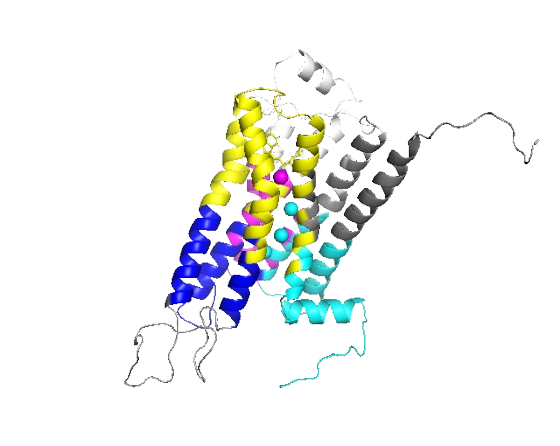
\includegraphics[width=\textwidth]{inactive.png}
      \caption{$\beta_2$ARのinactive状態において検出されたコミュニティ構造を色分けして示した図。各色と名付けたコミュニティは以下に表す:黒(start)、シアン(end)、白(helix)、ピンク(back)、グレー(loop)、黄色(ligand)、青(gprotein)。}
      \label{fig:inactive_water}
    \end{subfigure}
    \hspace{0.05\textwidth} % 図の間のスペース
    \begin{subfigure}{0.45\textwidth}
      \centering
      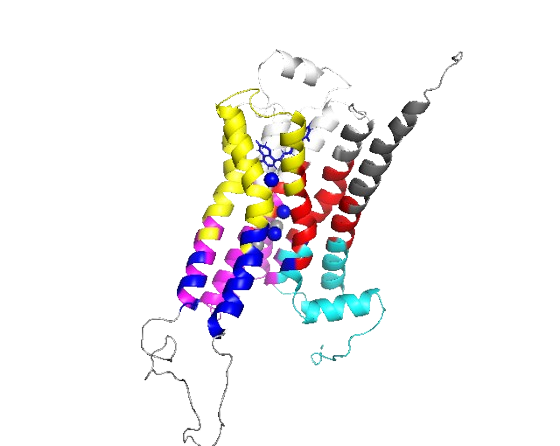
\includegraphics[width=\textwidth]{active.png}
      \caption{$\beta_2$ARのactive状態において検出されたコミュニティ構造を色分けして示した図。各色と名付けたコミュニティは以下に表す:黒(start)、シアン(end)、白(helix)、ピンク(back)、グレー(loop)、黄色(ligand)、青(gprotein)、赤(new)。}
      \label{fig:active_water}
    \end{subfigure}
    \caption{コミュニティ構造}
    \label{fig:water-all}
  \end{figure}

まず双方のコミュニティに共通することとして、リガンド結合部位と活性部位であるGタンパク質結合部位に対応する独立したコミュニティが、黄色(ligand)、青(gprotein)として検出された。
また図\ref{fig:inactive}から図\ref{fig:active}への変化として、青(gprotein)コミュニティの再編成が起きていることと、赤(new)コミュニティが新規に形成されたことが挙げられる。

青(gprotein)コミュニティと赤(new)コミュニティに属する残基の比較を行うと、以下のようになる。

%比較したtableを追加

active状態になると、青(gprotein)コミュニティにはリガンドと保存された結晶水3つ、赤(new)コミュニティにはモチーフが追加された。
%何のモチーフ

ここで、図\ref{fig:inactive}と図\ref{fig:active}で示されているネットワークの全体密度を計算する。
全体エッジ密度$D_{\text{global}}$の計算式は以下のように表される。

\[
W_{\text{actual}} = \sum_{(u, v) \in E} w(u, v)
\]

W_{\text{actual}}は実際のエッジ重みの合計である。
$E$は、グラフ内のエッジ集合を示す。
$w(u, v)$は、エッジ$(u, v)$の重みを示す。

\[
W_{\text{max}} = \sum_{i=1}^{N} \sum_{j=i+1}^{N} w(i, j)
\]

W_{\text{max}}は理論上可能な最大エッジ重みの合計である。
$N$は、グラフ内のノード数を示す。
$w(i, j)$は、ノード$i$と$j$の間のエッジ重みを示す。

\[
D_{\text{global}} = \frac{W_{\text{actual}}}{W_{\text{max}}}
\label{eq:global_density}
\]

最終的に、ネットワークの全体エッジ密度$D_{\text{global}}$は以上のように示される。

この式に基づいて、inactive構造とactive構造のネットワークの全体エッジ密度を計算すると、それぞれ以下のようになる。
\begin{itemize}
    \item inactive状態:\( Q = 0.3083 \)
    \item active状態:\( Q = :0.8579 \)
\end{itemize}

inactive状態は低い密度を示しており、最短距離が3\,\text{\AA}未満の残基ペアが相対的に少なかった。
active状態は、inactive状態に比べて高い全体エッジ密度を持っており、より多くの相互作用が存在することを示している。この結果は、活性状態におけるタンパク質の構造や機能がより密接に結びついていることを示唆している。

\subsection{コミュニティ内およびコミュニティ間のエッジ密度}
active状態で再編成されたコミュニティや新しく検出されたコミュニティの役割を定量的に分析するために、ネットワークの全体密度$D_{\text{global}}$の計算で用いた密度の概念を用いたさらなる計算を行った。
続いて、inactive状態とactive状態双方においてそれぞれコミュニティ内のエッジ密度、コミュニティ間のエッジ密度を計算した。

\subsubsection{コミュニティ内エッジ密度}
コミュニティ内エッジ密度$D_{\text{internal}}$の計算式は以下のように表される。

まずコミュニティごとにサブグラフを作成する。
ただしコミュニティ間のエッジは削除し、独立したコミュニティを表現している。
続いてコミュニティ内エッジ密度を計算する。

\[
D_{\text{internal}} = \frac{\sum_{(u,v) \in E_C} w_{uv}}{\sum_{(u,v) \in E_C} w_{uv}^{\text{max}}}
\label{eq:internal_density}
\]

ここで$E_C$はコミュニティ$C$内の全エッジの集合、$w_{uv}$はノード$u$とノード$v$の間の実際のエッジ重み、$w_{uv}^{\text{max}}$はノード$u$とノード$v$の間のエッジの最大可能重みである。
分子の\(\sum_{(u,v) \in E_C} w_{uv}\)はコミュニティに属するノード間に存在する実際のエッジの重みの合計を示している。
分母の \(\sum_{(u,v) \in E_C} w_{uv}^{\text{max}}\) は、そのコミュニティ内の全てのノードが完全に接続している場合のエッジの最大可能重みの合計を示している。
ただし、自己ループは除く。


コミュニティ内エッジ密度$D_{\text{internal}}$は、ネットワーク全体のエッジ密度を基準としてコミュニティ内のエッジ密度がネットワーク全体と比べて相対的にどれだけ高い(または低い)かを示し、コミュニティ内部でどれだけ密接に関連しているかを測定することを目的としている。
上記の式に基づいて、inactive構造とactive構造のコミュニティ内エッジ密度を計算すると、それぞれ以下のようになる。

\begin{figure}[htbp]
    \centering
    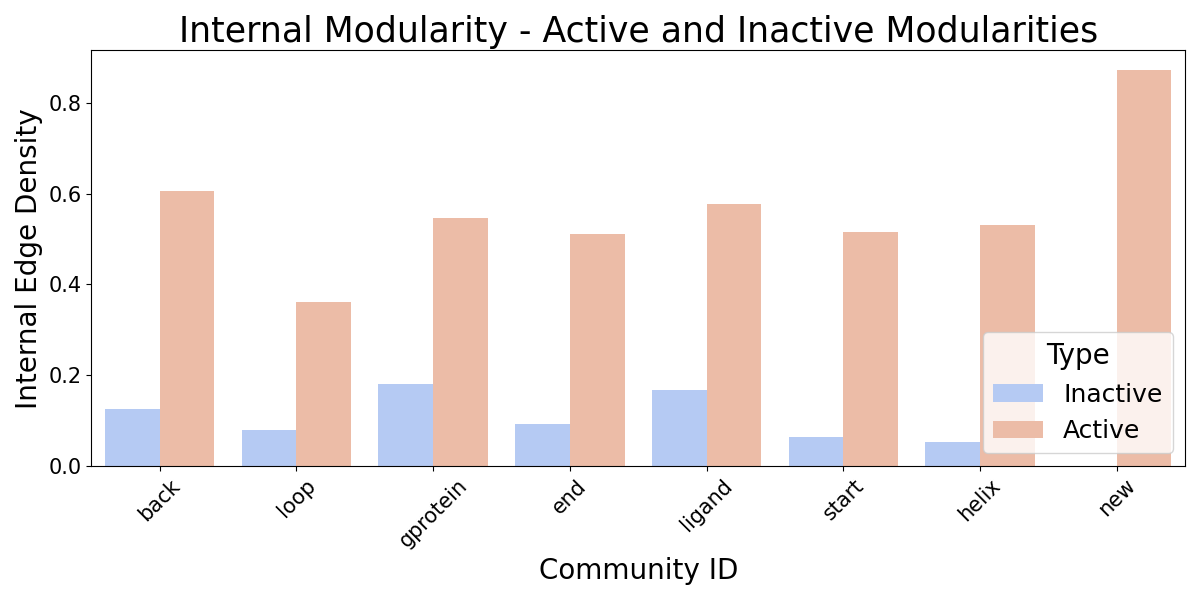
\includegraphics[width=0.8\textwidth]{internal_modularities.png}
    \caption{$\beta_2$ARのinactive状態とactive状態において検出されたコミュニティのコミュニティ内エッジ密度を示した図。コミュニティの名称は、図\ref{fig:inactive}と図\ref{fig:active}で名付けたものである。}
    \label{fig:internal}
\end{figure}

コミュニティ内エッジ密度$D_{\text{internal}}$の値は以下のように解釈される:
\begin{itemize}
    \item \( D_{\text{internal}} \) が 0 に近い:コミュニティ内のノード間の相互作用は希薄であり、結びつきが弱い。
    \item \( D_{\text{internal}} \) が 1 に近い:コミュニティ内のノード間には強い結びつきがあり、密に相互作用している。
\end{itemize}

inactive構造では、loop, newコミュニティのコミュニティ内エッジ密度が特に大きい値を示した。
一方でactive構造においては、全てのコミュニティのコミュニティ内エッジ密度が1.0付近という値を示し、特に強い結びつきを形成している構造であることがわかる。
inactive構造からactive構造への変化に着目すると、どのコミュニティも値が大幅に大きくなり、特にgproteinコミュニティが顕著であった。

\subsubsection{コミュニティ間エッジ密度}
コミュニティ間エッジ密度$D_{\text{inter}}$の計算式は以下のように表される。

\[
D_{\text{inter}} = \frac{\sum_{\substack{u \in C_i \\ v \in C_j}} w_{uv}}{\sum_{\substack{u \in C_i \\ v \in C_j}} w_{uv}^{max}}
\label{eq:inter_density}
\]

ここで$C_i$と$C_j$はそれぞれ異なるコミュニティ$i$と$j$、$w_{uv}$はノード$u$とノード$v$の間の実際のエッジ重み、$w_{uv}^{\text{max}}$はノード$u$とノード$v$の間のエッジの最大可能重みである。
分子の \sum_{\substack{u \in C_i \\ v \in C_j}} w_{uv} は異なるコミュニティに属するノード間の実際のエッジの重みの合計を示している。
分母の \sum_{\substack{u \in C_i \\ v \in C_j}} w_{uv}^{max} は、そのコミュニティ間の全てのノードが完全に接続している場合のエッジの最大可能重みの合計を示している。
ただし、自己ループは除く。

コミュニティ間エッジ密度は、異なるコミュニティ間のエッジの結びつきの強さを示しており、お互いにどれだけ相互作用が強いかを測定することを目的としている。
上記の式に基づいて、inactive構造とactive構造のコミュニティ間エッジ密度を計算すると、それぞれ以下のようになる。

\begin{figure}[htbp]
    \centering
    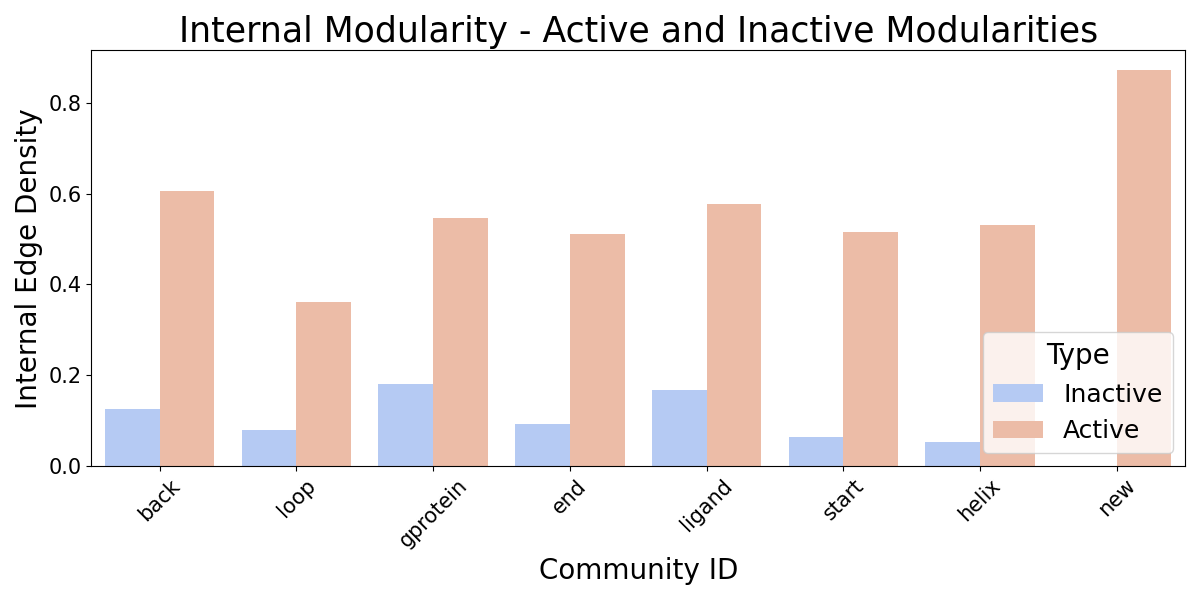
\includegraphics[width=0.8\textwidth]{internal_modularities.png}
    \caption{$\beta_2$ARのinactive状態とactive状態において検出されたコミュニティのコミュニティ間エッジ密度を示した図。コミュニティの名称は、図\ref{fig:inactive}と図\ref{fig:active}で名付けたものである。}
    \label{fig:internal}
\end{figure}

ただし、inactive状態とactive状態の双方でコミュニティ間エッジ密度が0だったコミュニティペアは、図から除外している。
該当するコミュニティペアはstart-loop、helix-loop、new-loopである。

コミュニティ間エッジ密度$Q$の値は以下のように解釈される:
\begin{itemize}
    \item \( Q \) が 0 に近い:コミュニティ間でエッジが少なく、各コミュニティがほぼ独立している。
    \item \( Q \) が 1 に近い:コミュニティ間で多数のエッジが存在し、コミュニティ間の結びつきが強い。
\end{itemize}

inactive状態では、コミュニティペアback-gprotein、helix-start、end-back、start-ligandが高い値を示した。
これらのコミュニティペアは隣り合っており、妥当な結果を示している。
active状態では、リガンド結合部位と活性部位の間に存在するコミュニティback, gprotein, ligand, newを含むコミュニティペアの値が特に顕著に高い値を示した。
特にnewコミュニティとペアを形成しているコミュニティペアに関しては、全て0.6以上と高い値を示した。
inactive構造からactive構造への変化に着目すると、リガンド結合部位と活性部位を結ぶ経路から離れているコミュニティペア(end,start)以外のどのコミュニティも、値が大幅に大きくなった。

\subsubsection{inactive状態とactive状態の全体密度、コミュニティ密度の考察}


\paragraph{密度に関わる3つの変数における、inactive状態からactive状態への変化}

ここまで計算したコミュニティ内エッジ密度、コミュニティ間エッジ密度、全体エッジ密度のinactive状態からactive状態への変化を示したのが以下の表である。
\begin{itemize}
    \item コミュニティ内エッジ密度:増加
    \item コミュニティ間エッジ密度:増加
    \item 全体エッジ密度:増加
\end{itemize}

inactive状態では、loopコミュニティやnewコミュニティにおいて相互作用がコミュニティ内部に局在化しており、gproteinコミュニティは内部の結びつきが弱かった。
またコミュニティ間のエッジ密度が低いため、各コミュニティの協調的な動きが抑制されている状態が観察された。
一方でactive状態になると、ほぼすべてのコミュニティ内の相互作用が増加し、コミュニティ間の相互作用も大幅に増加し、その結果全体密度も増加する状態が観察された。
特にnewコミュニティに関わるコミュニティペア間の相互作用の強さが特徴的であった。
まとめると、active状態になるとコミュニティ内部と間の相互作用が増加するようにコミュニティの再編成が起き、結果的に全体の協調的な動きが活性化している様子が見てとれる。
これらの結果から、分子全体の協調的な相互作用が増加し情報伝達の効率が向上するアロステリック遷移のメカニズムが示唆される。
またこの遷移において、activeで新たに形成されたnewコミュニティが、リガンド結合部位や活性部位であるGタンパク質結合部位間の情報伝達を促進する導管として働いている可能性がある。
%密度変化やnewコミュニティの重要性や生理的・機能的意義を、先行研究と交えて

\section{ノード削除によるactiveネットワーク接続性への影響}

あるノードがactiveネットワーク全体または所属するコミュニティの接続性に与える影響を定量化に評価するために、impact scoreという変数を導入した。
これは、特定のノードをactiveネットワークから削除した際に生じる全体エッジ密度とコミュニティ内エッジ密度の変化量を基に計算した。全体エッジ密度とコミュニティ内エッジ密度はそれぞれ前述の式(式 \ref{eq:global_density})と式(式 \ref{eq:internal_density})に従っている。
以降、全体エッジ密度の変化量をglobal impact score、コミュニティ内エッジ密度の変化量をcommunity impact scoreと表現する。

また、global impact scoreとcommunity impact scoreについて、Zスコアを算出することで影響の大小を統計的に評価する。
Zスコアは、あるデータ点で平均からどれだけ標準偏差の単位で離れているかを示す指標である。Zスコアの計算式は以下のとおりである。

\[
z = \frac{x - \mu}{\sigma}
\]

ここで$x$はデータ点の値、$\mu$はデータセットの平均、$\sigma$はデータセットの標準偏差を示している。
Zスコアの解釈は以下のとおりである。
\begin{itemize}
    \item \( z < 0 \):データ点は平均よりも小さい値である。
    \item \( z = 0 \):データ点は平均と一致している。
    \item \( z > 0 \):データ点は平均よりも大きい値である。
    \item \( z > 2 \):データ点は平均から2標準偏差以上離れており、全体の約2.5\%にあたるくらい高い値である。
\end{itemize}

\subsubsection{global impact score}
global impact scoreの変化量が大きかったノードのうち、Zスコアが2以上であったノードを昇順に並び替えたのが以下の表である。
\begin{table}[ht]
    \centering
    \begin{tabular}{|l|r|c|r|}
    \hline
    \textbf{Node} & \textbf{Global Impact Score} & \textbf{Community} & \textbf{Node type}\\
    \hline
    303 & 0.000775 & new & Ligand-Site \\
    62 & 0.000773 & new & Other \\
    66 & 0.000766 & new & Motif \\
    273 & 0.000753 & ligand & Motif \\
    111 & 0.000747 & new & Other \\
    96 & 0.000740 & back & Ligand-Site \\
    69 & 0.000739 & new & Motif \\
    107 & 0.000724 & new & Motif \\
    104 & 0.000683 & new & Ligand-Site \\
    108 & 0.000678 & ligand & Other \\
    58 & 0.000669 & helix & Other \\
    100 & 0.000647 & new & Ligand-Site \\
    105 & 0.000640 & back & Ligand-Site \\
    110 & 0.000635 & helix & Other \\
    339 & 0.000635 & end & Other \\
    114 & 0.000626 & helix & Other \\
    186 & 0.000622 & back & Ligand-Site \\
    342 & 0.000622 & end & Other \\
    \hline
    \end{tabular}
    \caption{Top 18 Nodes by Impact Score}
\end{table}

ここでCommunityの名称は、図\ref{fig:inactive}と図\ref{fig:active}で名付けたものである。
Node typeは以下の

上位10このうち7このノードがnewコミュニティに属しており、active構造で検出された新しいコミュニティが重要な役割を果たしていることが示唆された。
また、リガンド結合部位やnewコミュニティに属しているモチーフに関連するノードが多く、これらの領域が全体のネットワーク密度に強い影響を与えていることが示唆される。
%リガンド結合が受容体の活性化に伴う全体的な構造変化を引き起こすという既存の知見
%https://www.cosmobio.co.jp/aaas_signal/archive/ra-20200204-2.asp?utm_source=chatgpt.com

\subsubsection{community impact score}
community impact scoreが大きかったノードのうち、Zスコアが2以上であったノードを昇順に並び替えたのが以下の表である。
\begin{table}[ht]
    \centering
    \begin{tabular}{|l|r|c|r|}
    \hline
    \textbf{Node} & \textbf{Community Impact Score} & \textbf{Community} & \textbf{Node type}\\
    \hline
    346 & 0.002723 & gprotein & X-Water \\
    347 & 0.002642 & gprotein & X-Water \\
    349 & 0.002634 & gprotein & X-Water \\
    348 & 0.002609 & gprotein & X-Water \\
    343 & 0.002576 & gprotein & Ligand \\
    241 & 0.002372 & loop & Other \\
    1 & 0.002248 & start & Other \\
    258 & 0.002208 & gprotein & Gprotein-Site \\
    231 & 0.002121 & loop & Other \\
    259 & 0.002074 & gprotein & Other \\
    243 & 0.002047 & loop & Other \\
    236 & 0.001998 & loop & Other \\
    17 & 0.001990 & start & Other \\
    242 & 0.001974 & loop & Other \\
    345 & 0.001969 & gprotein & X-Water\\
    239 & 0.001962 & loop & Other \\
    2 & 0.001876 & start & Other \\
    222 & 0.001826 & loop & Other \\
    255 & 0.001815 &  gprotein & Motif \\
    339 & 0.001767 & end & Other \\
    217 & 0.001761 & loop & Gprotein-Site \\
    261 & 0.001746 & gprotein & Gprotein-Site \\
    \hline
    \end{tabular}
    \caption{Top 22 Nodes by Impact Score}
\end{table}
    
22このうち18このノードがgproteinコミュニティもしくはloopコミュニティに属しており、active状態において再編成を起こした2つのコミュニティ内の重要な結束性に寄与している可能性がある。
また、上位4つを保存された結晶水が占めていることから、これらがgタンパク質結合領域内で強い影響力を持つことを示している。
%Gタンパク質の活性化には、受容体の特定の構造変化が必要であり、これらの局所的な相互作用がそのプロセスを制御している可能性
%https://seikagaku.jbsoc.or.jp/10.14952/SEIKAGAKU.2022.940916/data/index.html?utm_source=chatgpt.com
%選択的活性化
%https://www.cosmobio.co.jp/aaas_signal/archive/ra-20200204-2.asp?utm_source=chatgpt.com


\subsubsection{global impact score、community impact scoreの考察}

global impact scoreが目立ったリガンド結合部位やモチーフに関わる残基はネットワーク全体の構造を保つ役割を果たしている。
つまり、リガンド結合部位やモチーフはネットワーク全体の「骨格」として、リガンド結合によるネットワーク全体の構造的再編成を引き起こし、アロステリックな影響を広げる重要な起点となっていることが示唆される。
community impact scoreが目立ったリガンドやgタンパク質結合部位、保存された結晶水に関わる残基は局所的なコミュニティ構造を保つ役割を果たしている。
つまり、リガンドやgタンパク質結合部位、保存された結晶水は局所的な「柔軟性」を提供し、Gタンパク質の結合やシグナル伝達の効率化を高めていることが示唆される。


%しかし
\section{シグナル伝達機構の考察}
以下は、完全に仮説なので、この仮説を裏付ける先行研究が発見されなければ、削除

ここまでinactive状態とactive状態におけるコミュニティ内密度とコミュニティ間密度、active状態のネットワークにおけるノードがactiveネットワーク全体または所属するコミュニティの接続性に与える影響について解析をしてきた。
これらの解析結果を踏まえると、以下のような段階的なシグナル伝達機構が考えられる。

まずリガンドがリガンド結合部位に結合すると、まず結合近傍の局所的なコミュニティ再編成が起きる。
この再編成はリガンドが高いcommunity impact scoreを示したことに反映されている。
続いて再編成されたリガンド結合部位が、局所的な変化を他のコミュニティへと伝播させることで、ネットワーク全体の構造変化が促進される。
この過程は、ligandコミュニティと他のコミュニティにおけるコミュニティ間密度が大幅に増加したことや、リガンド結合部位が高いglobal impact scoreを示したことに反映されている。
最後に、再編成されたネットワーク全体がgタンパク質結合部位や保存された結晶水などの局所的な結束性によって安定化され、シグナル伝達が効率的に進む。
この過程は、gproteinコミュニティのコミュニティ内密度が大幅に増加したことや、gproteinコミュニティに含まれる保存された結晶水が高いcommunity impact scoreを示したことに反映されている。

\chapter{考察}
\include{discussion}

\chapter{結論}
本研究では、$\beta$2ARのinactive状態およびactive状態におけるネットワーク構造を解析し、Louvain法を用いて検出されたコミュニティの特性を比較した。


まず検出されたコミュニティを比較すると、Gタンパク質結合部位が再編成され、新規のコミュニティが形成されていることが明らかになった。


続いてそれぞれのネットワークの全体エッジ密度、コミュニティ内エッジ密度、コミュニティ間エッジ密度を比較した。
全体エッジ密度に関しては、inactive状態では0.133、active状態では0.127となり、活性化によるTM6の外側への動きによるエッジの減少が影響していると考察された。


全てのコミュニティでコミュニティ内エッジ密度が増加し、新たに出現したnewコミュニティは0.87という高い値を示した。
コミュニティ間エッジ密度の解析では、
(gprotein,loop)(gprotein,ligand)(helix,ligand)(back,ligand)というリガンド結合部位からGタンパク質部位をつなぐ導線にあるコミュニティペアの相互作用が強化されており、
特に新しく生成されたnewコミュニティに関連するコミュニティペアは相対的に高い値を示した。
これらの結果は、active状態への遷移に伴う分子全体のネットワーク再編成が、
コミュニティ内部の相互作用を強化させるとともに、
情報伝達に関わる分子間の情報伝達の効率化を支える重要なメカニズムであることを示している。
特に、newコミュニティが形成されたことで、リガンド結合部位や活性部位であるGタンパク質結合部位間の情報伝達を促進する導管として働いている可能性があることが示唆された。


最後にノード削除が全体エッジ密度とコミュニティ内エッジ密度に与える影響の解析では、
リガンド結合部位やnewコミュニティに属しているモチーフに関するノードが全体エッジ密度に、
リガンドやgタンパク質結合部位、保存された結晶水がコミュニティ内エッジ密度に与える影響が大きくなった。
前者はネットワーク全体の「骨格」としてアロステリックな影響を広げる重要な起点となっていることが、
後者は局所的な「足場」を提供しGタンパク質の結合やシグナル伝達の効率化を高めていることが示唆された。

\section{今後の展望}
本研究ではノード間の距離を重みとした構造ネットワークを用いた。
しかし活性化によってダイナミクスや相互作用のみが変化したノードに関しては、構造ネットワークではその変化を捉えることが困難である。
そのため、構造のみならず、局所的なダイナミクスや相互作用も反映した変数である局所熱伝導度\cite{yamato2022computational}を重みとした物理的な熱拡散ネットワークの構築により、$\beta$2ARのアロステリー機構の解明をより詳細に理解することが期待できる。
%参考文献:熱伝導度
%https://pubs.acs.org/doi/10.1021/acs.jpcb.2c00958
また、Louvain法によるコミュニティ検出では、特定の時間スケールでの1つのコミュニティ分割しか検出しておらず、異なる時間スケールでの過渡現象を観察できない。
そのため、マルコフ安定性\cite{amor2014uncovering}のようなネットワーク内のさまざまなスケールに存在する多層コミュニティ構造を識別できる動力学ベースのマルチスケール方の導入が必要である。
%参考文献:マルコフ安定性
%https://pubs.rsc.org/en/content/articlehtml/2014/mb/c4mb00088a?casa_token=HGfB0iRp9w0AAAAA:3-CTB2Oe4qIicEKrQcC2P6ekaNArGHCwe3FlWDLugZpZvLBt1sOqi5ziQJed1dOzFS6kOYXHzWU-jQ

\chapter{謝辞}
学部3年次の生物物理セミナーからはじめ、3年間の研究の遂行にあたり、指導教官として終始多大なご指導を賜った、倭剛久先生に深謝致します。
研究室選びに迷っている中で学部3年次に出席した生物物理分野に興味を持ち、急遽研究室見学を受け入れてくださった時から今まで、生物物理に関する深い知識と経験に基づく多くの有益な助言をいただきました. 
木村明洋先生にも、講義やセミナー、研究室での議論を通じて、多くのご指導をいただきました。
またB研の皆様には、本研究の遂行にあたり多大なご助言、ご協力頂きました。
特に王婷婷氏、杉浦航氏、在田陽一氏には、右も左もわからなかった自分に、生物物理やシミュレーションの基礎をはじめ、私の疑問や悩みをたくさん解決していただきました。
大久保雄大氏、吉村風汰氏、大櫃丈氏には、研究室内発表時の議論を通じて多くの刺激をもらいました。

最後に、研究ができる環境を提供していただき、精神的な支えにもなっていただいた両親や祖父、姉に深く感謝いたします。

% 参考文献
\printbibliography[title=参考文献]

\end{document}
